\documentclass{aip-cp}

\usepackage[numbers]{natbib}
\usepackage{rotating}
\usepackage{graphicx}
\pdfmapfile{+txfonts.map}

%%%%%ДОБАВИЛ ДЛЯ РУССКОГО ТЕКСТА
\usepackage[utf8x]{inputenc}
\usepackage[english,russian]{babel}
\usepackage{cmap}
%%%%%


% Document starts
\begin{document}

% Title portion
\title{The Title Goes Here with Each Initial Letter Capitalized}

\author{Victor Gergel}
\author{Konstantin Barkalov\corref{cor1}}
%\eaddress[url]{http://www.aip.org}
\author{Ilya Lebedev}
%\eaddress{anotherauthor@thisaddress.yyy}

\affil{Lobachevsky State University of Nizhni Novgorod, Nizhni Novgorod, Russia.}
\corresp[cor1]{Corresponding author: konstantin.barkalov@itmm.unn.ru}

\maketitle


\begin{abstract}
Abstract.
\end{abstract}

% Head 1
\section{INTRODUCTION}

In the present paper, the methods for generating the global optimization test problems with non-convex constraints
\begin{eqnarray}
&\varphi(y^\ast)=\min{\left\{\varphi(y):y\in D, \; g_i(y)\leq 0, \; 1 \leq i \leq m\right\}}, \label{i_problem} \\
&D=\left\{y\in R^N: a_i\leq y_i \leq b_i, 1\leq i \leq N\right\} \label{D}
\end{eqnarray}
are considered. The objective function $\varphi(y)$ (henceforth denoted by $g_{m+1}(y)$) and the left-hand sides $g_i(y), \; 1\leq i \leq m,$ of the constraints are supposed to satisfy the Lipschitz condition
\[ \left|g_i(y')-g_i (y'')\right| \leq L_i \left\|y'-y'' \right\|, \; y',y''\in D, \; 1\leq i \leq m+1. \]
with the Lipschitz constants unknown a priori. The analytical formulae of the problem functions may be unknown, i.e. these ones may be defined by an algorithm for computing the function values in the search domain (so called ``black-box''-functions). It is supposed that even a single computing of a problem function value may be a time-consuming operation since it is related to the necessity of numerical modeling in the applied problems (see, for example, \cite{Menniti2008,Kvasov2015,Modorskii2017}).

The evaluation of efficiency of the developed methods is one of the key problems in the optimization theory and applications. Unfortunately, it is difficult to obtain any theoretical estimates in many cases. As a result, the comparison of the methods is performed by carrying out the computational experiments on solving some test optimization problems in most cases. In order to obtain a reliable evaluation of the efficiency of the methods, the sets of test problems should be diverse and representative enough. The problem of choice of the test problems has been considered in a lot of works (see, for example, \cite{Floudas1999,Gaviano2003,Ali2005,Addis2007}). Unfortunately, in many cases, the proposed sets contain a small number of test problems, and it is difficult to obtain the problems with desired properties. The most important drawback consists of the fact that the constraints are absent in the proposed test problems as a rule (or the constraints are relatively simple: linear, convex, etc.).



\section{Test problem classes}
A well-known approach to investigating and comparing the multiextremal optimization algorithms is based on testing these methods by solving a set of problems, chosen randomly from some specially designed class. 

%One generator for random samples of two-dimensional test functions has been described in \cite{Grishagin1978,Grishagin2016}. This generator produces two-dimensional functions according to the formula
%\begin{eqnarray} \nonumber \label{VAG}
%\varphi(y)= -&\left\{\left(\sum^{7}_{i=1}\sum^{7}_{j=1}A_{ij}g_{ij}(y)+B_{ij}h_{ij}(y)\right)^2+\right. \\
%&\left.\left(\sum^{7}_{i=1}\sum^{7}_{j=1}C_{ij}g_{ij}(y)+D_{ij}h_{ij}(y)\right)^2\right\}^{1/2},\\ \nonumber
%\end{eqnarray}
%where $g_{ij}(y)=\sin(i\pi y_1)\sin(j\pi y_2)$, $h_{ij}(y)=\cos(i\pi y_1)\cos(j\pi y_2)$, $y=(y_1,y_2)\in R^2, \; 0 \leq y_1,y_2 \leq 1$, and coefficients $A_{ij}, B_{ij}, C_{ij}, D_{ij}$  are taken uniformly in the interval $[-1,1]$.

Let us consider a scheme for constructing the generator GCGen (Global Constrained optimization problem Generator) which allows to generate the test global optimization problems with $m$ constraints. Obviously, one can generate $m+1$ functions, the first $m$ of these ones can be considered as the constraints and the $(m+1)$-th function -- as the objective one. However, in this case, the conditional global minimizer of the objective function is unknown, and the preliminary estimate of this one (for example, by scanning over a uniform grid) will be time-consuming. At the same time, one could not control the size of the feasible domain. In particular, the constraints might be incompatible, and the feasible domain might be empty. 

Below, the rules, which allow formulating the constrained global optimization problems so that:
\begin{itemize}
	\item one could control the size of feasible domain with respect to the whole domain of the parameters' variation;
	\item the global minimizer of the objective function would be known a priori taking into account the constraints;
	\item the global minimizer of the objective function without accounting for the constraints would be out of the feasible domain (with the purpose of simulating the behavior of the constraints and the objective function in the applied constrained optimization problems)
\end{itemize}
are proposed. 

The rules defining the operation of the generator of the constrained global optimization with the properties listed above consist in the following.

\begin{enumerate}
	\item Let us generate $m+1$ functions $f_j(y), y \in D, 1 \leq j \leq m+1,$ by some generating scheme (for instance, by using the formula (\ref{VAG})). The constraints will be constructed on the base of the first $m$ functions, the $(m+1)$-th function will serve for the construction of the objective function.
	\item In order to know the global minimizer in the constrained problem a priori, let us make it to be the same to the global minimizer in the unconstrained problem. To do so, let us perform a linear transformation of coordinates so that the global minimizers of the constraint functions $y_j^\ast, \; 1 \leq j \leq m,$ would transit into the minimizer of the objective function $y_{m+1}^\ast$. This way, the functions $\overline{f_j}(y), \; 1 \leq j \leq m,$ with the same point of extremum will be constructed.
		\item In order to control the size of the feasible domain, let us construct an auxiliary function (a combined constraint)
		\[
		H(y)=\max_{1 \leq j \leq m}{\overline{f_j}(y)}
		\]
and compute its values in the nodes of a uniform grid in the domain $D$; the number of the grid nodes in the conducted experiments should be big enough (in our experiments it was $\min \left\{10^7, 10^{2N} \right\}$). Then, let us find the maximum and minimum values of the function $H(y)$ in the grid nodes, $H_{max}$ and $H_{min}$, respectively, and construct a characteristic $s(i)$ -- the number of points, in which the values of $H(y)$ fall into the range 
\[
\left[H_{min},H_{min}+i\frac{H_{max}-H_{min}}{100}\right], \; 1 \leq i \leq 100 .
\]
Then, the functions 
\[
\overline{f_j}(y) \leq q = H_{min}+i\frac{H_{max}-H_{min}}{100}, \; 1 \leq j \leq m,
\]
where $i$ is selected to be the minimal one satisfying the inequality
\[
\Delta \leq \frac{s(i)}{s(100)}
\]
will construct a problem with the feasible domain occupying the fraction $\Delta, \; 0<\Delta<1,$ of the whole search domain.
\item 
The test problem of global constrained optimization can be stated as follows
\[
\min\left\{ \varphi(y):y \in D, \; g_j(y)= \overline{f_j}(y)-q \leq 0, \; 1 \leq j \leq m \right\}
\]
where 
%$\varphi(y)=f_{m+1}(y)$. This problem will possess all declared properties (the fraction of the feasible domain will consist $\Delta$ of the whole search domain and the global minimizer of the constrained problem will be known).
%\item 
%In order to complicate the test constrained problem the form of the objective function can be expanded by the expression
\[
\varphi(y) = f_{m+1}(y)-\beta\sum_{j=1}^m\max\left\{0,\overline{f_j}(y) -q \right\}^\alpha,
\]
where $\alpha$ is a positive integer number and $\beta>0$ is selected in such a way as to provide the global minimum location of the function $\varphi(y)$ in the infeasible part of the search domain $D$. For instance, to guarantee this property the value of $\beta$ can be set as follows
\[
\beta>(h_{max}-h_{min})/(H_{max}-q)^\alpha,
\]
where $h_{max}$ and $h_{min}$ are the maximum and minimum values of the function $f_{m+1}(y)$ respectively.
\end{enumerate}

\Russian
Одним из важных свойств, характеризующих прикладные задачи условной оптимизации, является расположение условного минимума на границе feasible domain. При генерации задач по схеме, описанной в \cite{Gergel2017}, условный минимум будет, вообще говоря, находиться внутри feasible domain. Поэтому в новой версиии генератора задач была добавлена возможность как смещения условного минимума на границу, так и выбора числа активных ограничений в нем.

Смещение условного минимума на границу feasible domain осуществляется следующим образом.
\begin{enumerate}
	\item Генерируется задача с произвольным расположением условного минимума $\overline{y}$;
	\item Из точки $\overline{y}$ с заданным шагом $h$ осуществляется покоординатный поиск допустимой точки $y^*$, для которой хотя бы одно из ограничений является активным, т.е. существует такой номер $j, 1 \leq j\leq m$, что $\left|g_j(y^*)\right| \leq \delta$. 
	\item Полученное грубое значение $y^*$ уточняется локальным методом. 
	\item Выполняется преобразование координат, переводящее точку $\overline{y}$ в точку $y^*$. Тем самым целевая функция достигает своего минимума на границе feasible domain. 
\end{enumerate}

Отметим, что так как поиск точки $y^*$ осуществляется по каждой координате в отдельности, то трудоемкость поиска будет возрастать линейно при увеличении размерности задачи.

В случае, если нужно сгенерировать задачу с заданным числом $S$ активных ограничений в точке условного минимума, то тогда правило 2 меняется следующим образом 
\begin{enumerate}
	\item В области поиска строится uniform grid с числом точек $\min \left\{10^7, 10^{2N} \right\}$, в каждой из которых вычисляются значения ограничений. 
	\item Определяется множество точек $\{y^t\}$, в которых активными являются $S$ ограничений; т.е. существуют такие номера $j_1, ...,j_S$, что $\left|g_{j_s}(y^t)\right|\leq \delta, \; 1\leq s \leq S$. В случае отсутствия такой точки, генерируется задача с произвольным числом активных ограничений и пользователь информируется об этом.
	\item Выбирается точка $y^* = \min_{t} \{\left\|\overline{y} - y^t\right\|\}$. Полученное грубое значение $y^*$ уточняется локальным методом. 
\end{enumerate}


\section{Numerical results}

As an illustration, the level lines of the objective functions and the zero-level lines of the constraints for problems constructed on the base of functions (\ref{VAG}) with $\alpha = 3, \beta = 1$ and the volume fractions of the feasible domains $\Delta = 0.4, 0.6$ are shown in Fig.~\ref{fig:VAG}. The feasible domains are highlighted by green. The change of volume and, at the same time, the increase of complexity of the feasible domains are seen clearly. Fig.~\ref{fig:VAG} (a,b) also shows the points of 628 and 764 trials, correspondingly, performed by the \textit{index method} for solving constrained global optimization problems until the required accuracy $\epsilon=10^{-2}$ was achieved. The conditional optimizer is shown as a red point and the best estimation of the optimizer is shown as a blue point.

The index method has been proposed and developed in \cite{Strongin2000,Sergeyev2001,Barkalov2002}. The approach is based on a separate accounting for each constraint of the problem and is not related to the use of the penalty functions. According to the rules of index method, every iteration includes a sequential checking of fulfillment of the problem constraints at this point. The first occurrence of violation of any constraint terminates the trial and initiates the transition to the next iteration. This allows: (i) accounting for the information on each constraint separately and (ii) solving the problems, in which the function values may be undefined out of the feasible domain. It should be noted, that the index method can be efficiently parallelized for accelerators \cite{Barkalov2015,Barkalov2016}.

\begin{figure}
\begin{minipage}{0.5\linewidth}
\center{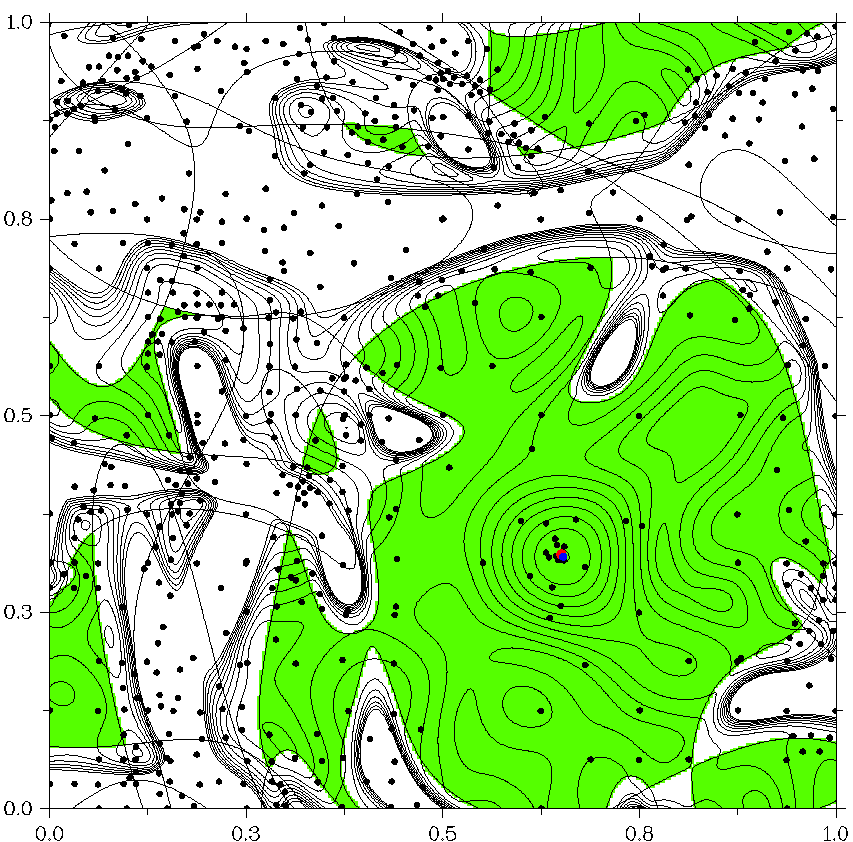
\includegraphics[width=1.0\linewidth]{vag_04.png} \\ (a)}
\end{minipage}
\hfill
\begin{minipage}{0.5\linewidth}
\center{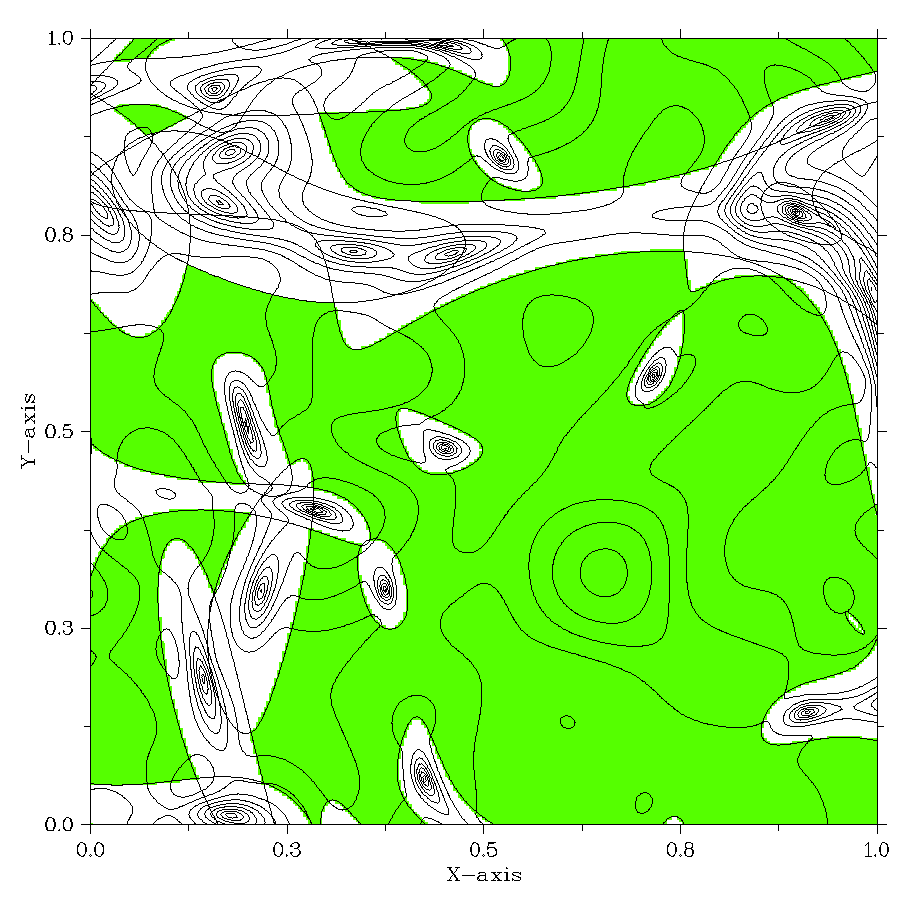
\includegraphics[width=1.0\linewidth]{vag_06.png} \\ (b)}
\end{minipage}
\caption{The problems based on functions (\ref{VAG}) }
\label{fig:VAG}
\end{figure}


\section {Conclusion}

This paper considers the method for generating global optimization test problems with non-convex constraints that allows:
\begin{itemize}
	\item to control the size of feasible domain with respect to the whole domain of the parameters' variation;
	\item to known a priori the conditional global minimizer of the objective function;
	\item to generate the unconditional global minimizer of the objective function out of the feasible domain (to simulate the constraints and objective function in the applied optimization problems).
\end{itemize}

The demonstration of the developed approach in application to well-known index method for solving complex multiextremal optimization problems with non-convex constraints is considered.

The developed approach allows generating any number of test global optimization problems with non-convex constraints for performing multiple computational experiments in order to obtain a reliable evaluation of the efficiency of the developed optimization algorithms.

% Acknowledgement
\section{ACKNOWLEDGMENTS}
This research was supported by the Russian Science Foundation, project No 16-11-10150.

% References

%\nocite{*}
\bibliographystyle{aipnum-cp}%
\bibliography{LeGo}%


\end{document}
